%%% LaTeX Template: Article/Thesis/etc. with colored headings and special fonts
%%%
%%% Source: http://www.howtotex.com/
%%% Feel free to distribute this template, but please keep to referal to http://www.howtotex.com/ here.
%%% February 2011
%%%
%%% Modified October 2015 by CDM

%%%  Preamble
\documentclass[11pt,letterpaper]{article}
\usepackage[margin=1.0in]{geometry}
\usepackage[T1]{fontenc}
\usepackage[bitstream-charter]{mathdesign}
\usepackage[latin1]{inputenc}					
\usepackage{amsmath}						
\usepackage{xcolor}
\usepackage{cite}
\usepackage{hyphenat}
\usepackage{graphicx}
\usepackage{float}
\usepackage{subfigure}
\usepackage{sectsty}
\usepackage[compact]{titlesec} 
\usepackage[tablegrid]{vhistory}
\allsectionsfont{\color{accentcolor}\scshape\selectfont}

%%% Definitions
\definecolor{accentcolor}{rgb}{0.0,0.0,0.5} 
\newcommand{\teamname}{Team Hawt Wheels}
\newcommand{\productname}{Smart Cart}
\newcommand{\coursename}{CSE 4316: Senior Design I}
\newcommand{\semester}{Spring 2016}
\newcommand{\docname}{Project Charter}
\newcommand{\department}{Department of Computer Science \& Engineering}
\newcommand{\university}{The University of Texas at Arlington}
\newcommand{\authors}{David Harvey \\ Dennis Otieno \\ Peggy Soh \\ Brian Wong \\ Or Zoarets}

%%% Headers and footers
\usepackage{fancyhdr}
	\pagestyle{fancy}						% Enabling the custom headers/footers
\usepackage{lastpage}	
	% Header (empty)
	\lhead{}
	\chead{}
	\rhead{}
	% Footer
	\lfoot{\footnotesize \teamname \ - \semester}
	\cfoot{}
	\rfoot{\footnotesize page \thepage\ of \pageref{LastPage}}	% "Page 1 of 2"
	\renewcommand{\headrulewidth}{0.0pt}
	\renewcommand{\footrulewidth}{0.4pt}

%%% Change the abstract environment
\usepackage[runin]{abstract}			% runin option for a run-in title
%\setlength\absleftindent{30pt}			% left margin
%\setlength\absrightindent{30pt}		% right margin
\abslabeldelim{\quad}	
\setlength{\abstitleskip}{-10pt}
\renewcommand{\abstractname}{}
\renewcommand{\abstracttextfont}{\color{accentcolor} \small \slshape}	% slanted text

%%% Start of the document
\begin{document}

%%% Cover sheet
{\centering \huge \color{accentcolor} \sc \textbf{\department \\ \university} \par}
\vspace{1 in}
{\centering \huge \color{accentcolor} \sc \textbf{\docname \\ \coursename \\ \semester} \par}
\vspace{0.5 in}
\begin{figure}[h!]
	\centering
   	
\includegraphics[width=0.60\textwidth]{images/smart_cart}
\end{figure}
\vspace{0.5 in}
{\centering \huge \color{accentcolor} \sc \textbf{\teamname \\ \productname} \par}
\vspace{0.5 in}
{\centering \large \sc \textbf{\authors} \par}
\newpage


%\vspace{1 in}
%\centerline{January 13th, 2012}
%\newpage

%%% Revision History
\begin{versionhistory}
  	\vhEntry{0.1}{02.10.2016}{DH, DO, PS, BW, OZ}{document creation}
  	\vhEntry{0.2}{02.17.2016}{DH, DO, PS, BW, OZ}{proof-read document}
\end{versionhistory}
\newpage

%%% Table of contents
\tableofcontents
\newpage

%%% List of figures and tables (optional)
\listoffigures
%\listoftables
\newpage

%%% Agile project charter sections
\section{Vision}
Our vision is to create the platform for an autonomous cart to assist educators by helping to transport and power various items from one place to another. The Smart Cart shall help ease the burden of having to make multiple trips and allow educators to use their time more efficiently. The cart shall also help ensure quality delivery of materials and serve to be part of the University of Texas at Arlington’s outreach program.

\section{Mission}
The mission of our project is to work as a team to design and develop a Smart Cart that will provide assistance by being an autonomous carrier. The cart needs to be able to do the following things: 
\begin{itemize}
	\item Follow a "master" to the designated destination
	\item Avoid collision with obstacles such as walls and other people
	\item Include an integrated power supply
	\item Holonomic mobility
\end{itemize}

The following list is how we will approach the project to achieve the items mentioned above:
\begin{itemize}
	\item Research on algorithms of how the cart will follow the "master" (lasers, colors or heat signature)
	\item Research the hardware modules (Omni wheels, motors, Intel RealSense, Kinect, Sonar, Stepper)
	\item Research on using Python or C++ and openCV for processing images if needed
	\item Use Google Drive, GitHub and LaTeX for documentation and collaboration
	\item Use GroupMe for team communication
\end{itemize}
\section{Success Criteria}
For the Smart Cart to be successful, it must satisfy the following criteria:
\begin{itemize}
	\item The total cost of the project shall not exceed \$800 USD. 
	\item The cart shall follow the master from one destination to another.
	\item The cart shall avoid collision with obstacles.
	\item The cart shall be able to move in any direction.
	\item The cart shall provide a power source.
	\item The cart shall be used by at least one educator.
	\item The cart shall be used in UTA's outreach program.
\end{itemize}
\newpage

%%% Remaining project charter sections
\section{Background}
Autonomous robots that are able to do hard manual labor are increasing in demand as they are able to outperform a human. Not only do they not tire, they can carry much heavier loads than a human. The Smart Cart is aimed at educators primarily to help them transport their teaching materials from one location to another. Some may wonder why there is a need for an autonomous cart if they can just push the cart itself. The purpose of the cart is not only allow educators to carry more equipment with little or no effort, the cart will also provide an integrated power supply. This allows the educators to be prepared for classes and demonstrations by keeping their equipment charged. Educators can also bring the cart out and provide demonstrations outside where there are often no outlets nearby. Such scenarios will be ideal for outreach programs. 

\section{Related Work}
In the past decade, research and development on autonomous carriers have become very popular and high in demand. Most of its applications are used in large manufacturing warehouses to move large, heavy objects, while other applications are to improve quality of life by providing assistance. Today, there are many autonomous robots and carriers available as open-source as well as commercial products. Some organizations even hold competitions for building such robots. The following are some robots that are closely related to our work:
\begin{itemize}
	\item Whole Foods has a motorized grocery cart prototype. The grocery cart follows customers around the store and tracks their shopping lists \cite{Welch}. 
	\item AGVSystems has automatic guided carts for material transportation and assembly line tasks. They follow a tape guided path \cite{AGC}.
	\item The Intelligent Ground Vehicle Competition is an annual robotics competition where students design and build autonomous ground vehicles that overcome several challenges \cite{IGVC}. 
\section{System Overview}
This section should describe the overall structure of your software system. Think of it as the strategy for how you will build the system. An architectural "layer" is the top-level logical view, or an abstraction, of your design. Layers should be composed of related elements of similar capabilities, and should be highly independent of other layers, but should have very clearly defined interfaces and interactions with other layers. Each layer should be identified individually and should be unique as to its function and purpose within the system. This section should also contain the high-level block diagram of the layers, as shown in the example below, as well as detailed descriptions of the functions of each layer.

\begin{figure}[h!]
	\centering
 	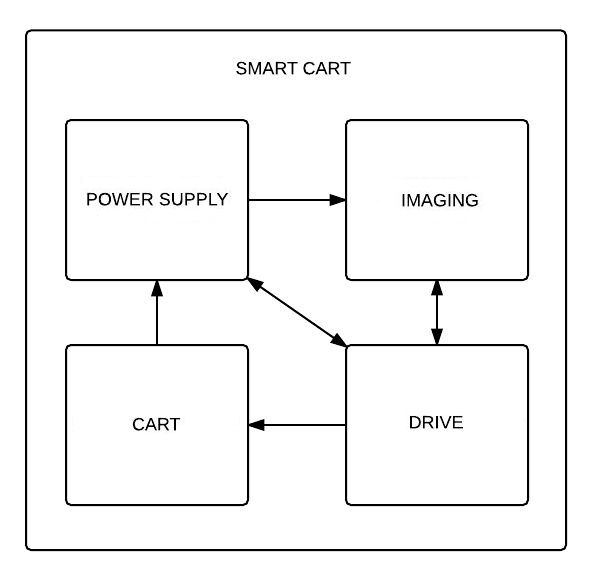
\includegraphics[width=0.60\textwidth]{images/system_overview}
 \caption{A simple architectural layer diagram}
\end{figure}


\subsection{Power Supply Layer Description}
Each layer should be described separately in detail. Descriptions should include the features, functions, critical interfaces and interactions of the layer. The description should clearly define the services that the layer provides. Also include any conventions that your team will use in describing the structure: naming conventions for layers, subsystems, modules, and data flows; interface specifications; how layers and subsystems are defined; etc.

\subsection{Cart Layer Description}
Each layer should be described separately in detail. Descriptions should include the features, functions, critical interfaces and interactions of the layer. The description should clearly define the services that the layer provides. Also include any conventions that your team will use in describing the structure: naming conventions for layers, subsystems, modules, and data flows; interface specifications; how layers and subsystems are defined; etc.

\subsection{Crab Drive Layer Description}
Each layer should be described separately in detail. Descriptions should include the features, functions, critical interfaces and interactions of the layer. The description should clearly define the services that the layer provides. Also include any conventions that your team will use in describing the structure: naming conventions for layers, subsystems, modules, and data flows; interface specifications; how layers and subsystems are defined; etc. 

\subsection{Imaging and Navigation Description}
Each layer should be described separately in detail. Descriptions should include the features, functions, critical interfaces and interactions of the layer. The description should clearly define the services that the layer provides. Also include any conventions that your team will use in describing the structure: naming conventions for layers, subsystems, modules, and data flows; interface specifications; how layers and subsystems are defined; etc. 
\section{Roles \& Responsibilities}
Despite official roles, our team is flexible with the distribution of work. The following are the official titles:
\begin{itemize}
	\item Project Owner/Team Leader: Or Zoarets
	\item Scrum Master: Dennis Otieno
	\item Documentation Master: Peggy Soh
	\item Hardware Tech: Brian Wong
	\item Logistics Expert: David Harvey
\end{itemize}
Team Leader/Project Owner Responsibilities: The Project Owner shall communicate between the project team members and other stakeholders, manage customer expectations and the budget.

Scrum Master Responsibilities: The Scrum Master shall remove any impediments that are obstructing any progression towards a sprint goal and keep all team members focused.

Documentation Master: The Documentation Master shall maintain all documentations and backlogs for the team.

Together as a team, our responsibilities are to perform our individual tasks as assigned and communicate to each other the progress of the project. If any issues arise, the Scrum Master will work to resolve the issues. 
\section{Facilities \& Equipment}
Our main facility will be the Senior Design Lab at UTA's Engineering Research Building, room 208. Other facilities that we may utilize will be the FabLab and school library. The equipment available to us are the school computers and the 3D printers. Other equipment that we will be using are detailed in the system overview section of this document.
\section{Cost Proposal}
\subsection{Preliminary Budget}
We have a budget of \$800 which is provided by the University of Texas at Arlington.
\section{Documentation \& Reporting}
\subsection{Project Charter}
The project charter shall be a key document for our project. This document defines the objectives, scope and structure for the design and development of the Smart Cart. The document will also show the schedule for sprints and establish the roles and responbilities for each team member. 

\subsection{Product Backlog}
The prodcut backlog will establish the initial requirements for the Smart Cart. The product backlog will be updated to reflect any requirements changes. All team members are responsible for checking the backlog to ensure that they are aware of the changes. All changes wil be documented and explained in this document.

\subsection{Sprint Planning}
All members of the team are required to attend to every sprint-planning meeting. The meetings will focus on completing tasks that will further progress the project. Documentations will be updated if necessary during sprint-plannings to keep everyone updated. The team will also define the sprint backlog and set the schedule for the sprint. Each sprint will be between 2 to 4 weeks.

\subsubsection{Sprint Goal}
The sprint goal is a descripion of what the team will be working towards for that sprint. This enables all team members to work towards the same goal. As the project progresses, the sprint goal will change.

\subsubsection{Sprint Backlog}
The sprint backlog is a list of tasks defined by the Scrum Master during a sprint team meeting. The tasks are split and assigned to each team member based on their strengths. This ensures that there will be progress towards the goal of each sprint. Each team member will then track the amount of hours they spent working on their tasks. New items will be added to the backlog for future sprints.

\subsubsection{Task Breakdown}
In order to complete certain tasks of the sprint backlog, the tasks will be broken down into small subtasks. Splitting the work load will ensure that each team member will complete their assigned work to the best of their abilities. Each individual is also responsible for researching and getting assistance if needed. The team will meet semi-weekly to ensure that all members are on track towards the sprint goal.

\subsection{Sprint Burndown Charts}
During each sprint, the burndown chart will change as the project progresses. The spreadsheet will have a list of tasks the estimated amount of time the team should spend on each task and the actual amount of time spend. In order to keep track of the sprint goal progress, the sprint burndown chart will be uploaded to the Google Drive folder shared by the team. This will ensure that all team members can track their progress and stay on track towards the sprint goal. An example of a sprint burndown chart is shown in Figure 1.

\begin{figure}[h!]
    \centering
    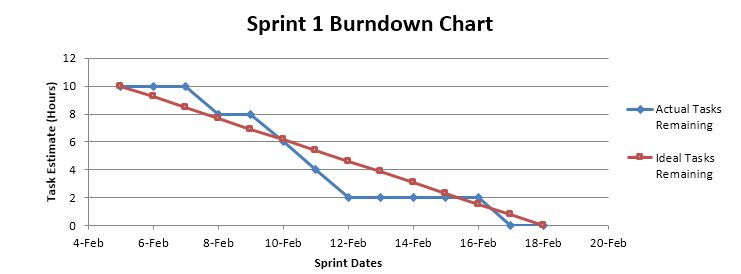
\includegraphics[width=0.80\textwidth]{images/chart}
    \caption{Sprint 1 Burndown Chart}
\end{figure}

\subsection{Sprint Retrospective}
During the sprint retrospective, the Scrum Master will debrief the team on the previous sprint session. The discussion will include improvements that could be made and other issues that need to be addressed if neccessary. This will help ensure that future sprints will be more productive and successful.

\subsection{Individual Status Reports}
Throughout the project, each team member is required to complete an individual status report. Each individual team member will record the tasks they have completed or are currently working on, the number of hours spent on each tasks and their future plans for the next sprint. If any unexpected tasks occurs, it will also be recorded.

\subsection{Engineering Notebooks}
Each team member is required to keep an Engineering notebook for the project. The notebook will contain details of each group meeting and any important ideas a team member finds. Any related work that is done outside of group time will also be recorded in the notebook. These notebooks are crucial for each team member since it is a legal document that tracks the teams' progress. 

\subsection{Closeout Materials}
\subsubsection{System Prototype}
During the development cycle, the team will develop a functioning prototype of the Smart Cart. As the project progresses, modifications to the prototype will be performed. All testing related to the project will be performed on the prototype. 

\subsubsection{Project Poster}
The project poster will include details of our project such as our vision, mission, and success criteria. This poster will be useful for presenting our project at UTA's outreach program.

\subsubsection{Demo Video}
The team will make a video to demonstrate the project. The video will explain how the cart will operate and the Smart Cart will demonstrate its intended functions.

\subsubsection{Source Code}
The source code will be stored on GitHub so the team can work on the software at their own pace. At this time, the project will be programmed in C++.

\subsubsection{Source Code Documentation}
The team will keep detailed documentation in the source code for the project. The purpose of the source code documentation is to explain the functions. This will allow future teams to easily understand the source code and make modification to the product.

\subsubsection{Hardware Schematics}
This project involves interfacing multiple hardware devices (Intel RealSense, Omni Wheels, Stepper motors), a camera module, electronic components and a power supply. The schematic diagram of the product will be the vital documentation that the team will provide.

\subsubsection{CAD files}
The team currently does not anticipate to have any CAD files. If any 3D printing is to be done later on, we will use the opensource GrabCad to find relevant files.

\subsubsection{User Manual}
The team will provide a user manual to explain how the Smart Cart will work. It will include details on how to power on, operate and power off the cart. It will also contain safety concerns and precautions.
\newpage

%%% References
\bibliographystyle{plain}
\bibliographystyle{reference/IEEEtran_custom}
\bibliography{reference/refs}{}

\end{document}
